\begin{frame}{$\bar{K}N$ interaction (Kaonic hydrogen puzzle)}
  \small
  \begin{tabular}{cc}
    \begin{minipage}{0.5\hsize}
      \begin{figure}
        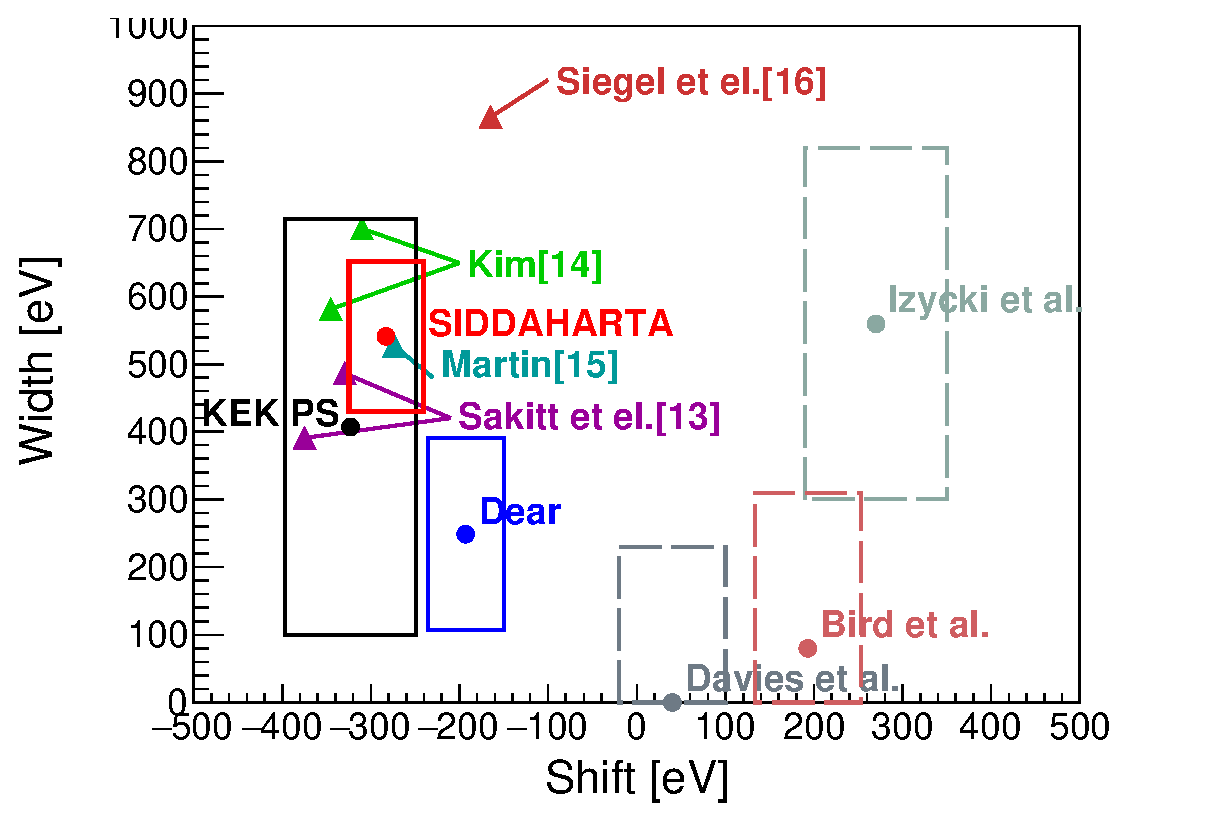
\includegraphics[width=6cm]{../pic/Dron/KN_int_map.eps}
      \end{figure}
    \end{minipage}
    \begin{minipage}{0.5\hsize}
      Deser-Trueman formula
      \begin{equation*}
        \Delta E_1^s -\frac{i}{2}\Gamma_1 = -2\alpha^3\mu_c^2a_{K^- p}
      \end{equation*}
      {\bf 1960's-1980's}\\
      \hspace{3mm} 1980 M. Izycki et al., \\
      \hspace{13mm} Z. Phys. A 297, 11 \\
      \hspace{3mm} 1979 J. D. Davies et al.,\\
      \hspace{13mm} Phys. Lett. B {\bf 83}, 55 \\      
      \hspace{3mm} 1983 P. M. Bird et al., \\
      \hspace{13mm} Nucl. Phys. A {\bf 404}, 482 \\
    \end{minipage}
  \end{tabular}
  \\
  \hspace{25mm} {\normalsize \bf Improve by usage of gasses target }
  \vspace{3mm} \\  
  \hspace{10mm} 1997 M. Iwasaki et el., Phys. Rev. Lett. {\bf 78}, 3067 {\bf KEK PS} \\
  \hspace{10mm} 2005 G. Beer et el., Phys. Rev. Lett. {\bf 94}, 212302 {\bf Dear} \\
  \hspace{10mm} 2011 M. Bazzi et el., Phys. Lett. B {\bf 704}, 113 {\bf SHIDDARTA} \\
  \hspace{20mm} $\Rightarrow$ Using as $\bar{K}N$ Constraint
\end{frame}
